\documentclass[tikz]{standalone}
\usetikzlibrary{shapes.callouts}
\tikzset{
    level/.style = {
        ultra thick,
        black,
    },
    connect/.style = {
        dashed,
        black
    },
    notice/.style = {
        draw,
        rectangle callout,
        callout relative pointer={#1}
    },
    label/.style = {
        text width=2cm
    }
}
\begin{document}
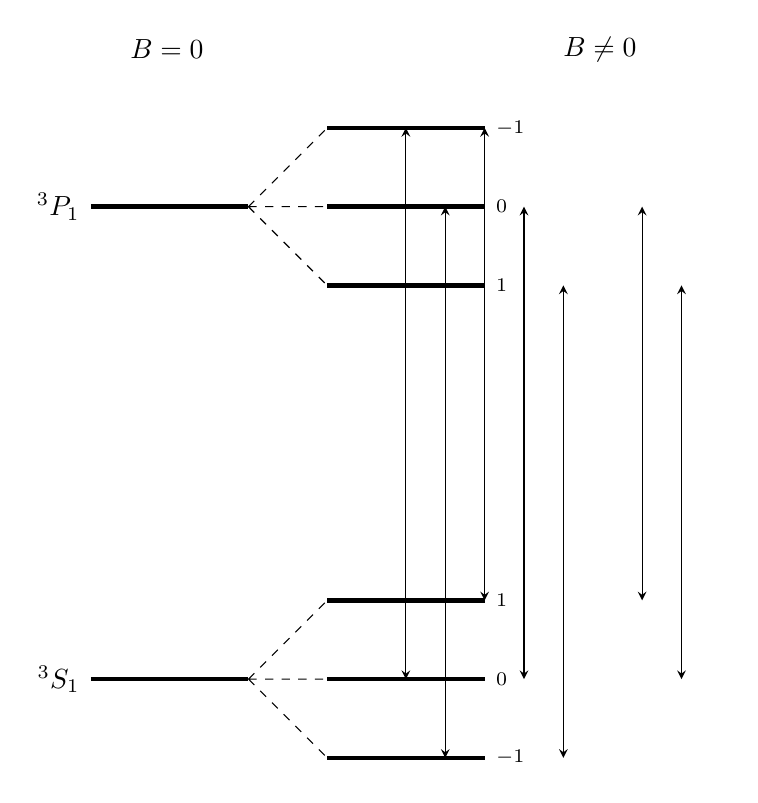
\begin{tikzpicture}
    % Draw all levels
    \draw[level] (0,+3) node[left] {$^3P_1$} -- (2,+3);
    \draw[level] (0,-3) node[left] {$^3S_1$} -- (2,-3);

    \draw[connect] (2,+3) -- (3,+4) (2,+3) -- (3,+3) (2,+3) -- (3,+2);
    \draw[connect] (2,-3) -- (3,-4) (2,-3) -- (3,-3) (2,-3) -- (3,-2);

    \draw[level] (3,+2) -- (5,+2) node[right] {\scriptsize $ 1$};
    \draw[level] (3,+3) -- (5,+3) node[right] {\scriptsize $ 0$};
    \draw[level] (3,+4) -- (5,+4) node[right] {\scriptsize $-1$};
    \draw[level] (3,-2) -- (5,-2) node[right] {\scriptsize $ 1$};
    \draw[level] (3,-3) -- (5,-3) node[right] {\scriptsize $ 0$};
    \draw[level] (3,-4) -- (5,-4) node[right] {\scriptsize $-1$};

    % Draw arrows
    \draw [stealth-stealth](4,+4) -- (4,-3);
    \draw [stealth-stealth](4.5,+3) -- (4.5,-4);
    %
    \draw [stealth-stealth](5,+4) -- (5,-2);
    \draw [stealth-stealth](5.5,+3) -- (5.5,-3);
    \draw [stealth-stealth](6,+2) -- (6,-4);
    %
    \draw [stealth-stealth](7,+3) -- (7,-2);
    \draw [stealth-stealth](7.5,+2) -- (7.5,-3);


    % Draw labels
    \node[label] at (1.5,5) {$B = 0$};
    \node[label] at (7,5) {$B \neq 0$};
\end{tikzpicture}
\end{document}
